\documentclass[11pt]{article}
\usepackage{geometry}                
\geometry{letterpaper}                   

\usepackage[english]{babel}	
\usepackage{graphicx}
\usepackage{german}
\usepackage[utf8]{inputenc} 
\usepackage{fancyhdr}
\usepackage{tabularx}
\usepackage{amssymb}
\usepackage{epstopdf}
\usepackage{natbib}
\usepackage{amssymb, amsmath}
\usepackage{float}
\usepackage{amsmath}

\DeclareGraphicsRule{.tif}{png}{.png}{`convert #1 `dirname #1`/`basename #1 .tif`.png}

%\title{Title}
%\author{Name 1, Name 2}
%\date{date} 

\begin{document}



\thispagestyle{empty}

\begin{center}
\includegraphics[width=5cm]{ETHlogo.eps}

\bigskip


\bigskip


\bigskip


\LARGE{ 	Lecture with Computer Exercises:\\ }
\LARGE{ Modelling and Simulating Social Systems with MATLAB\\}

\bigskip

\bigskip

\small{Project Report}\\

\bigskip

\bigskip

\bigskip

\bigskip


\begin{tabular}{|c|}
\hline
\\
\textbf{\LARGE{Swiss Rail Network Formation with}}\\
\textbf{\LARGE{Physarum Polycephalum}}\\
\\
\hline
\end{tabular}
\bigskip

\bigskip

\bigskip

\LARGE{Lucas Böttcher \\ Simon Roth \\ Gabriela Schär}



\bigskip

\bigskip

\bigskip

\bigskip

\bigskip

\bigskip

\bigskip

\bigskip

Zurich\\
December 2012\\

\end{center}



\newpage

%%%%%%%%%%%%%%%%%%%%%%%%%%%%%%%%%%%%%%%%%%%%%%%%%

\newpage
\section*{Agreement for free-download}
\bigskip


\bigskip


\large We hereby agree to make our source code for this project freely available for download from the web pages of the SOMS chair. Furthermore, we assure that all source code is written by ourselves and is not violating any copyright restrictions.

\begin{center}

\bigskip


\bigskip


\begin{tabular}{@{}p{6cm}@{}p{6cm}@{}@{}p{6cm}@{}}
\begin{minipage}{6cm}
 \large Lucas Böttcher

\end{minipage}
& 
\begin{minipage}{6cm}
\large Simon Roth

\end{minipage}
&
\begin{minipage}{6cm}
\large Gabriela Schär

\end{minipage}
\end{tabular}
\end{center}
\newpage

%%%%%%%%%%%%%%%%%%%%%%%%%%%%%%%%%%%%%%%



% IMPORTANT
% you MUST include the ETH declaration of originality here; it is available for download on the course website or at http://www.ethz.ch/faculty/exams/plagiarism/index_EN; it can be printed as pdf and should be filled out in handwriting


%%%%%%%%%% Table of content %%%%%%%%%%%%%%%%%

\tableofcontents

\newpage

%%%%%%%%%%%%%%%%%%%%%%%%%%%%%%%%%%%%%%%



\section{Abstract}

As most of the countries, Switzerland is growing. Cities are getting more inhabitants, growing together or arising new. With more people living in the cities and generally in Switzerland, more people will use the public transport system and the railroad network has to grow and develop. In this case, the main goal of this project is to simulate the Swiss railroad network depending on population growth to see where the systems should be improved.~\\
The network is simulated like a biological model, based on Physarum polycephalum. This slime mold is a large single-celled amoeboid organism that forages for food sources. To maximize the searched area, it explores it's environment with a relatively continous foraging margin. It's forming different junctions and nodes to reduce the overall length of the connecting network \cite{network_tokyo}. And this principle is adapted to the main transport lines in Switzerland.

 


\section{Individual contributions}

\section{Introduction and Motivations}

\section{Description of the Model}

The model is inspired of the physarum polycephalum and the way it's searching for food. The organism have been subjected to succsessice rounds of evolutionary selection and have found an appropiate balance between efficiency, cost and resilience. The plasmodium contains a network of tubes, which enables chemical signals and nutrients to circulate through the organism. If some of the tubes have found food sources, this implies a positive feedback to the system. This tubes are getting thicker so the flux of nutrients increase. Other tubes which don't connect to a food sources are shrinking and tend to disapear. because there is no flux available. Experiments showed two empirical rooles. First tubes with no connection to a source disappear and second, if there are two tubes connecting the same source, the longer one disappears. This led to useful approaches to problem-solving like optimization of railroad systems or networks in general.~\\
~\\
The mathematical model is based on \textit{Physarum solver: A biologically inspired method of road-network navigation} \cite{network_model}. Figure \ref{fig:schema} shows the concept of the mathematical model. There are different nodes. First two nodes corresponding to the food sources ($N_1$ and $N_2$) and other nodes ($N_3$, $N_4$ ... $N_j$). The junction between the node $N_i$ and $N_j$ is denoted as $M_{ij}$.

\begin{figure}[H]
	\centering
	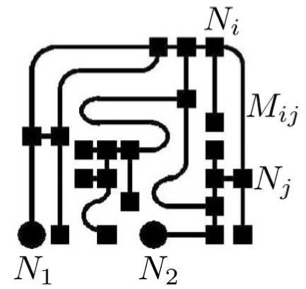
\includegraphics[width=0.4\textwidth]{schema.jpg}
	\caption{Concept of the mathematical model. Squares represent ordinary nodes, circles 			represent food sources, each line represent a junction}
	\label{fig:schema}
\end{figure}

The variable $Q_{ij}$ stands for the flux through the junction $M_{ij}$ from $N_i$ to $N_j$. The flux $Q_{ij}$ is given by an approximately Poiseuille flow where $p_i$ is a pressure at the node $N_i$, $L_{ij}$ is the length and $D_{ij}$ is the conductivity of the junction $M_{ij}$ :

\begin{equation}
	\label{eq:1}
	Q_{ij}=\frac{D_{ij}}{L_{ij}}\left(p_i-p_j\right)
\end{equation}

By considering Kirchhoff's law at each node, there is:

\begin{equation}
	\label{eq:2}
	\sum_{i} Q_{ij}=0 \,\,\,\, \mathrm{if} \left(j\ne 1,2\right)
\end{equation}

$N_1$ is assumed as a source node and $N_2$ as a sink and $I_0$ represent the flux from the source node and is in this model constant. It followed:

\begin{equation}
	\label{eq:3}
	\sum_{i} Q_{i1}+I_0=0, \,\,\,\, \sum_{i} Q_{i2}-I_0=0
\end{equation}

To describe the thickness of the junctions we assumed that the conductivity $D_{ij}$ changes in time according to the flux $Q_{ij}$:

\begin{equation}
	\label{eq:4}
	\frac{dD_{ij}}{dt}=f\left(\mid Q_{ij} \mid \right)-D_{ij}
\end{equation}

where $f\left(\mid Q \mid \right)$ is a increasing function with $f(0)=0$. Here $f\left(\mid Q \mid \right)$ is given by:

\begin{equation}
	\label{eq:5}
	f\left(\mid Q \mid \right)=\frac{\mid Q \mid^\gamma }{1+\mid Q \mid^\gamma}
\end{equation}

The network Poisson equation for the pressure is derived from the equations (\ref{eq:1}), (\ref{eq:2}) and (\ref{eq:3}) as followed:

\begin{equation}
	\label{eq:6}
	\sum_{i} \frac{D_{ij}}{L_{ij}}\left(p_i-p_j\right)= \begin{cases}
										-I_0 & \mathrm{for}\,\, j=1,\\
										I_0 & \mathrm{for} \,\,j=2,\\
										0 & \mathrm{otherwise}
										\end{cases}
\end{equation}

All $p_i$'s can be determined by solving the equation system (\ref{eq:6}) wenn setting $p_2=0$ as a basic pressure level. With this also each $Q_{ij}$ is obtained. They're definend bay the $D_{ij}$'s and $L_{ij}$'s  at each time step. Conductivity is closely related to the thickness of the junctions and so when a conductivity of a junction is zero, it disappears.

\section{Implementation}

\section{Simulation Results and Discussion}

\section{Summary and Outlook}



\bibliographystyle{plain}
\bibliography{matlabbib}






\end{document}  



 
